% Options for packages loaded elsewhere
% Options for packages loaded elsewhere
\PassOptionsToPackage{unicode}{hyperref}
\PassOptionsToPackage{hyphens}{url}
\PassOptionsToPackage{dvipsnames,svgnames,x11names}{xcolor}
%
\documentclass[
  11pt,
]{article}
\usepackage{xcolor}
\usepackage[margin=1in]{geometry}
\usepackage{amsmath,amssymb}
\setcounter{secnumdepth}{5}
\usepackage{iftex}
\ifPDFTeX
  \usepackage[T1]{fontenc}
  \usepackage[utf8]{inputenc}
  \usepackage{textcomp} % provide euro and other symbols
\else % if luatex or xetex
  \usepackage{unicode-math} % this also loads fontspec
  \defaultfontfeatures{Scale=MatchLowercase}
  \defaultfontfeatures[\rmfamily]{Ligatures=TeX,Scale=1}
\fi
\usepackage{lmodern}
\ifPDFTeX\else
  % xetex/luatex font selection
\fi
% Use upquote if available, for straight quotes in verbatim environments
\IfFileExists{upquote.sty}{\usepackage{upquote}}{}
\IfFileExists{microtype.sty}{% use microtype if available
  \usepackage[]{microtype}
  \UseMicrotypeSet[protrusion]{basicmath} % disable protrusion for tt fonts
}{}
\usepackage{setspace}
\makeatletter
\@ifundefined{KOMAClassName}{% if non-KOMA class
  \IfFileExists{parskip.sty}{%
    \usepackage{parskip}
  }{% else
    \setlength{\parindent}{0pt}
    \setlength{\parskip}{6pt plus 2pt minus 1pt}}
}{% if KOMA class
  \KOMAoptions{parskip=half}}
\makeatother
% Make \paragraph and \subparagraph free-standing
\makeatletter
\ifx\paragraph\undefined\else
  \let\oldparagraph\paragraph
  \renewcommand{\paragraph}{
    \@ifstar
      \xxxParagraphStar
      \xxxParagraphNoStar
  }
  \newcommand{\xxxParagraphStar}[1]{\oldparagraph*{#1}\mbox{}}
  \newcommand{\xxxParagraphNoStar}[1]{\oldparagraph{#1}\mbox{}}
\fi
\ifx\subparagraph\undefined\else
  \let\oldsubparagraph\subparagraph
  \renewcommand{\subparagraph}{
    \@ifstar
      \xxxSubParagraphStar
      \xxxSubParagraphNoStar
  }
  \newcommand{\xxxSubParagraphStar}[1]{\oldsubparagraph*{#1}\mbox{}}
  \newcommand{\xxxSubParagraphNoStar}[1]{\oldsubparagraph{#1}\mbox{}}
\fi
\makeatother


\usepackage{longtable,booktabs,array}
\usepackage{calc} % for calculating minipage widths
% Correct order of tables after \paragraph or \subparagraph
\usepackage{etoolbox}
\makeatletter
\patchcmd\longtable{\par}{\if@noskipsec\mbox{}\fi\par}{}{}
\makeatother
% Allow footnotes in longtable head/foot
\IfFileExists{footnotehyper.sty}{\usepackage{footnotehyper}}{\usepackage{footnote}}
\makesavenoteenv{longtable}
\usepackage{graphicx}
\makeatletter
\newsavebox\pandoc@box
\newcommand*\pandocbounded[1]{% scales image to fit in text height/width
  \sbox\pandoc@box{#1}%
  \Gscale@div\@tempa{\textheight}{\dimexpr\ht\pandoc@box+\dp\pandoc@box\relax}%
  \Gscale@div\@tempb{\linewidth}{\wd\pandoc@box}%
  \ifdim\@tempb\p@<\@tempa\p@\let\@tempa\@tempb\fi% select the smaller of both
  \ifdim\@tempa\p@<\p@\scalebox{\@tempa}{\usebox\pandoc@box}%
  \else\usebox{\pandoc@box}%
  \fi%
}
% Set default figure placement to htbp
\def\fps@figure{htbp}
\makeatother

\ifLuaTeX
  \usepackage{luacolor}
  \usepackage[soul]{lua-ul}
\else
  \usepackage{soul}
\fi




\setlength{\emergencystretch}{3em} % prevent overfull lines

\providecommand{\tightlist}{%
  \setlength{\itemsep}{0pt}\setlength{\parskip}{0pt}}



 
\usepackage[]{biblatex}
\addbibresource{references.bib}


\makeatletter
\@ifpackageloaded{tcolorbox}{}{\usepackage[skins,breakable]{tcolorbox}}
\@ifpackageloaded{fontawesome5}{}{\usepackage{fontawesome5}}
\definecolor{quarto-callout-color}{HTML}{909090}
\definecolor{quarto-callout-note-color}{HTML}{0758E5}
\definecolor{quarto-callout-important-color}{HTML}{CC1914}
\definecolor{quarto-callout-warning-color}{HTML}{EB9113}
\definecolor{quarto-callout-tip-color}{HTML}{00A047}
\definecolor{quarto-callout-caution-color}{HTML}{FC5300}
\definecolor{quarto-callout-color-frame}{HTML}{acacac}
\definecolor{quarto-callout-note-color-frame}{HTML}{4582ec}
\definecolor{quarto-callout-important-color-frame}{HTML}{d9534f}
\definecolor{quarto-callout-warning-color-frame}{HTML}{f0ad4e}
\definecolor{quarto-callout-tip-color-frame}{HTML}{02b875}
\definecolor{quarto-callout-caution-color-frame}{HTML}{fd7e14}
\makeatother
\makeatletter
\@ifpackageloaded{caption}{}{\usepackage{caption}}
\AtBeginDocument{%
\ifdefined\contentsname
  \renewcommand*\contentsname{Table of contents}
\else
  \newcommand\contentsname{Table of contents}
\fi
\ifdefined\listfigurename
  \renewcommand*\listfigurename{List of Figures}
\else
  \newcommand\listfigurename{List of Figures}
\fi
\ifdefined\listtablename
  \renewcommand*\listtablename{List of Tables}
\else
  \newcommand\listtablename{List of Tables}
\fi
\ifdefined\figurename
  \renewcommand*\figurename{Figure}
\else
  \newcommand\figurename{Figure}
\fi
\ifdefined\tablename
  \renewcommand*\tablename{Table}
\else
  \newcommand\tablename{Table}
\fi
}
\@ifpackageloaded{float}{}{\usepackage{float}}
\floatstyle{ruled}
\@ifundefined{c@chapter}{\newfloat{codelisting}{h}{lop}}{\newfloat{codelisting}{h}{lop}[chapter]}
\floatname{codelisting}{Listing}
\newcommand*\listoflistings{\listof{codelisting}{List of Listings}}
\makeatother
\makeatletter
\makeatother
\makeatletter
\@ifpackageloaded{caption}{}{\usepackage{caption}}
\@ifpackageloaded{subcaption}{}{\usepackage{subcaption}}
\makeatother
\usepackage{bookmark}
\IfFileExists{xurl.sty}{\usepackage{xurl}}{} % add URL line breaks if available
\urlstyle{same}
\hypersetup{
  pdftitle={William's Comments},
  pdfauthor={William Clinton Co},
  colorlinks=true,
  linkcolor={blue},
  filecolor={Maroon},
  citecolor={Blue},
  urlcolor={Blue},
  pdfcreator={LaTeX via pandoc}}


\title{William's Comments}
\usepackage{etoolbox}
\makeatletter
\providecommand{\subtitle}[1]{% add subtitle to \maketitle
  \apptocmd{\@title}{\par {\large #1 \par}}{}{}
}
\makeatother
\subtitle{Tariffs, Trade and Tumult Canada's challenges ahead}
\author{William Clinton Co}
\date{July 3, 2025}
\begin{document}
\maketitle
\begin{abstract}
This document provides comments on Prof.~Michael B. Devereux's
presentation, ``Tariffs, Trade, and Tumult: Canada's Challenges Ahead,''
delivered at the Pender Whistler Investment Conference on July 9, 2025.
\end{abstract}

\renewcommand*\contentsname{Table of contents}
{
\hypersetup{linkcolor=}
\setcounter{tocdepth}{3}
\tableofcontents
}

\setstretch{1.5}
\section{Introduction}\label{sec-introduction}

Overall, the presentation is strong. The comments below focus on minor
corrections to improve clarity and consistency, such as rephrasing for
clarity, adding explanatory sentences, increasing font size, labeling
axes, and ensuring consistent formatting.

\section{Comments}\label{comments}

\subsection{Slide 3}\label{slide-3}

\begin{figure}

\centering{


\includegraphics[width=0.7\linewidth,height=\textheight,keepaspectratio,page=3]{bean.pdf}

}

\caption{\label{fig-slide3}Slide 3}

\end{figure}%

Roadmap:

\begin{enumerate}
\def\labelenumi{\arabic{enumi}.}
\item
  The postwar trading system
\item
  The US tariff shock
\item
  \begin{tcolorbox}[enhanced jigsaw, opacitybacktitle=0.6, rightrule=.15mm, opacityback=0, breakable, titlerule=0mm, colback=white, left=2mm, leftrule=.75mm, colbacktitle=quarto-callout-tip-color!10!white, colframe=quarto-callout-tip-color-frame, toptitle=1mm, bottomtitle=1mm, coltitle=black, title=\textcolor{quarto-callout-tip-color}{\faLightbulb}\hspace{0.5em}{Maybe say}, bottomrule=.15mm, arc=.35mm, toprule=.15mm]

  \st{The logic of tariffs} maybe say ``Evaluating Tariffs''

  \end{tcolorbox}
\item
  The impact on Canada
\item
  The way forward?
\end{enumerate}

\subsection{Slide 4}\label{slide-4}

\begin{figure}

\centering{


\includegraphics[width=0.7\linewidth,height=\textheight,keepaspectratio,page=4]{bean.pdf}

}

\caption{\label{fig-slide4}Slide 4}

\end{figure}%

Evolution of the global trading system

\begin{itemize}
\item
  \begin{tcolorbox}[enhanced jigsaw, opacitybacktitle=0.6, rightrule=.15mm, opacityback=0, breakable, titlerule=0mm, colback=white, left=2mm, leftrule=.75mm, colbacktitle=quarto-callout-tip-color!10!white, colframe=quarto-callout-tip-color-frame, toptitle=1mm, bottomtitle=1mm, coltitle=black, title=\textcolor{quarto-callout-tip-color}{\faLightbulb}\hspace{0.5em}{Gave better background on GATT}, bottomrule=.15mm, arc=.35mm, toprule=.15mm]

  GATT \textbf{\emph{(General Agreement on Tariffs and Trade)}} set up
  in 1947 under US leadership

  \end{tcolorbox}
\item
  Tari rates over 20\% in 1950s..
\item
  \ldots.
\end{itemize}

\subsection{Slide 5}\label{slide-5}

\begin{figure}

\centering{


\includegraphics[width=0.7\linewidth,height=\textheight,keepaspectratio,page=5]{bean.pdf}

}

\caption{\label{fig-slide5}Slide 5}

\end{figure}%

\begin{tcolorbox}[enhanced jigsaw, opacitybacktitle=0.6, rightrule=.15mm, opacityback=0, breakable, titlerule=0mm, colback=white, left=2mm, leftrule=.75mm, colbacktitle=quarto-callout-tip-color!10!white, colframe=quarto-callout-tip-color-frame, toptitle=1mm, bottomtitle=1mm, coltitle=black, title=\textcolor{quarto-callout-tip-color}{\faLightbulb}\hspace{0.5em}{Suggestion}, bottomrule=.15mm, arc=.35mm, toprule=.15mm]

\begin{enumerate}
\def\labelenumi{\arabic{enumi}.}
\tightlist
\item
  Label the axis
\item
  Maybe confusing because there are two points being made.

  \begin{enumerate}
  \def\labelenumii{\arabic{enumii}.}
  \tightlist
  \item
    World trade growth vs GDP growth

    \begin{itemize}
    \tightlist
    \item
      show mean of World Trade and mean of GDP comparison
    \end{itemize}
  \item
    Trade and Post War success

    \begin{itemize}
    \tightlist
    \item
      show pre war growth against post war growth
    \end{itemize}
  \end{enumerate}
\end{enumerate}

\pandocbounded{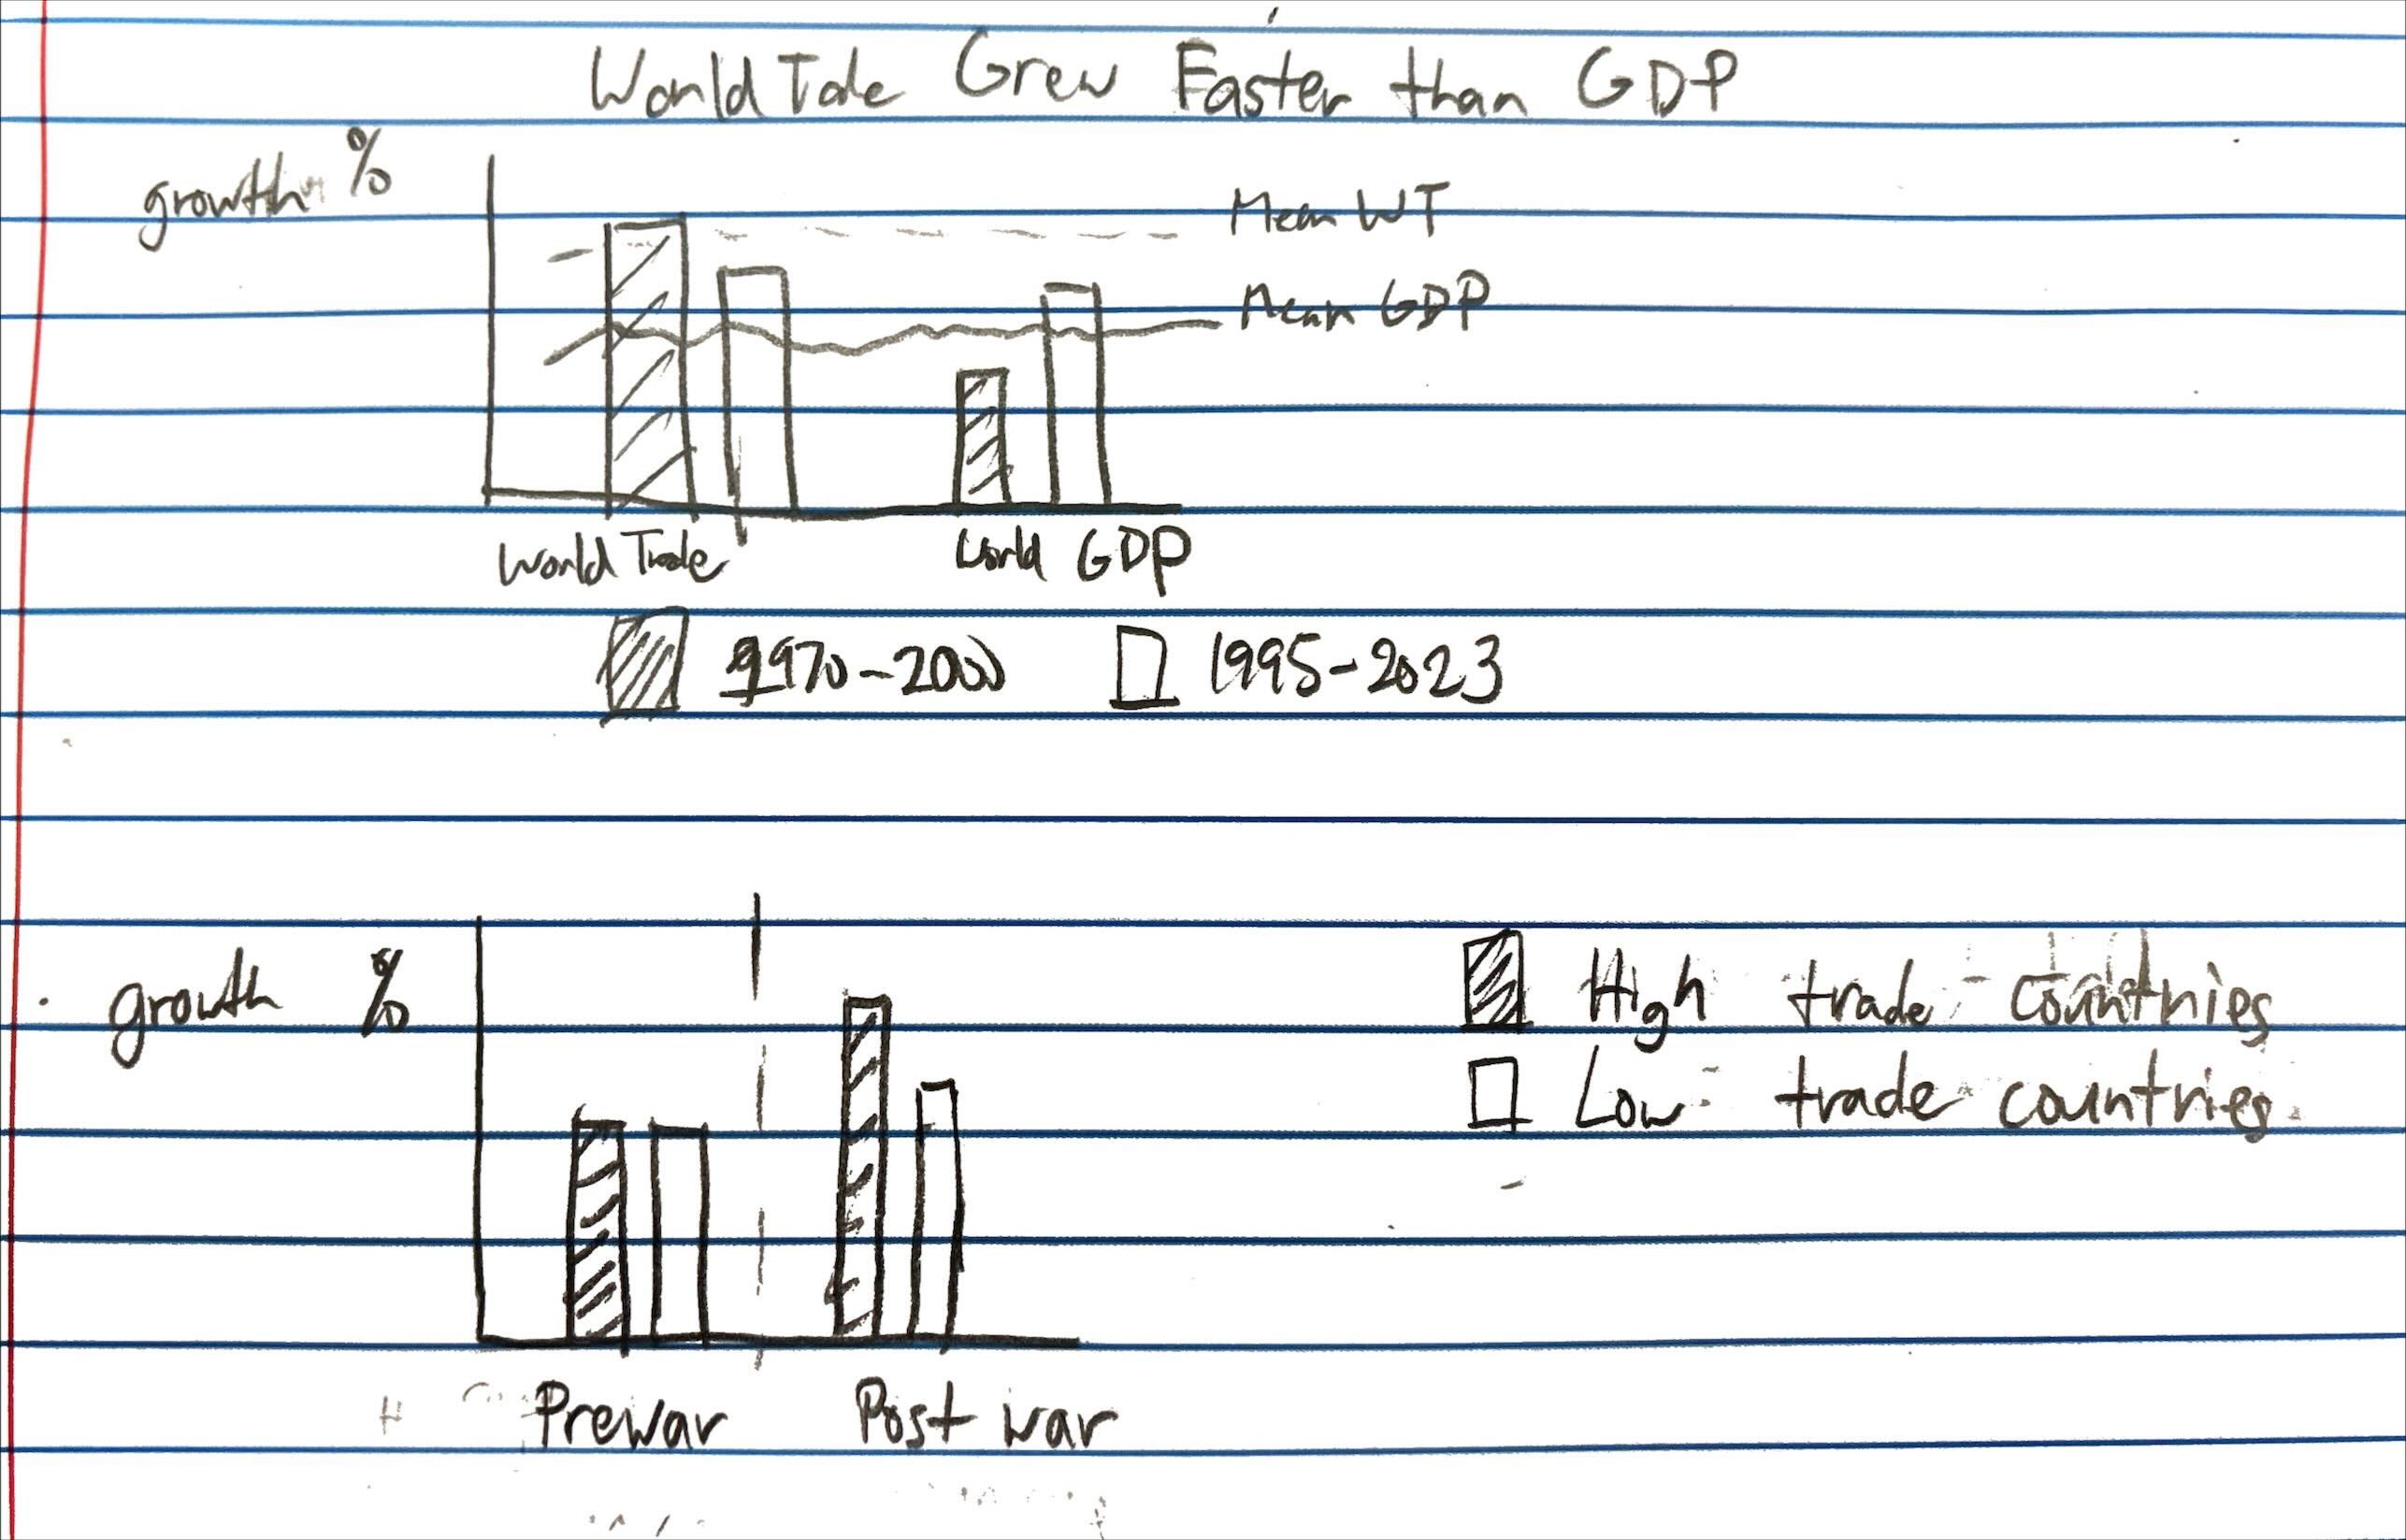
\includegraphics[keepaspectratio]{images/clipboard-4219370577.jpeg}}

\end{tcolorbox}

\subsection{Slide 6}\label{slide-6}

\begin{figure}

\centering{


\includegraphics[width=0.7\linewidth,height=\textheight,keepaspectratio,page=6]{bean.pdf}

}

\caption{\label{fig-slide6}Slide 6}

\end{figure}%

\begin{tcolorbox}[enhanced jigsaw, opacitybacktitle=0.6, rightrule=.15mm, opacityback=0, breakable, titlerule=0mm, colback=white, left=2mm, leftrule=.75mm, colbacktitle=quarto-callout-tip-color!10!white, colframe=quarto-callout-tip-color-frame, toptitle=1mm, bottomtitle=1mm, coltitle=black, title=\textcolor{quarto-callout-tip-color}{\faLightbulb}\hspace{0.5em}{Suggestion}, bottomrule=.15mm, arc=.35mm, toprule=.15mm]

add a small bullet point explanation of trade diversion

ie.

\begin{description}
\item[Trade Diversion]
when trade is diverted from a more efficient exporter towards a less
efficient one.
\end{description}

\end{tcolorbox}

\subsection{Slide 7}\label{slide-7}

\begin{figure}

\centering{


\includegraphics[width=0.7\linewidth,height=\textheight,keepaspectratio,page=7]{bean.pdf}

}

\caption{\label{fig-slide7}Slide 7}

\end{figure}%

\begin{tcolorbox}[enhanced jigsaw, opacitybacktitle=0.6, rightrule=.15mm, opacityback=0, breakable, titlerule=0mm, colback=white, left=2mm, leftrule=.75mm, colbacktitle=quarto-callout-tip-color!10!white, colframe=quarto-callout-tip-color-frame, toptitle=1mm, bottomtitle=1mm, coltitle=black, title=\textcolor{quarto-callout-tip-color}{\faLightbulb}\hspace{0.5em}{Tip}, bottomrule=.15mm, arc=.35mm, toprule=.15mm]

Indicate new ``chapter'' with a chapter slide. i.e.

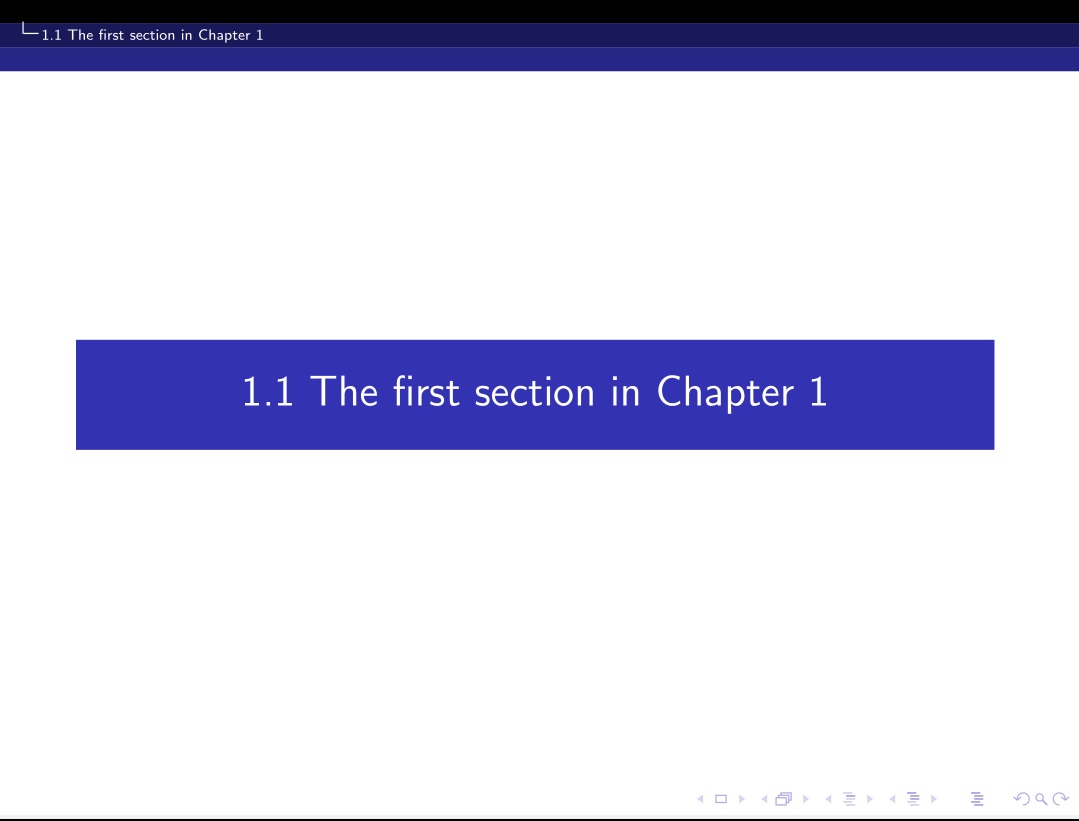
\includegraphics[width=3.98958in,height=\textheight,keepaspectratio]{images/clipboard-2994615373.jpeg}

\end{tcolorbox}

\subsection{Slide 8}\label{slide-8}

\begin{figure}

\centering{


\includegraphics[width=0.7\linewidth,height=\textheight,keepaspectratio,page=8]{bean.pdf}

}

\caption{\label{fig-slide8}Slide 8}

\end{figure}%

\begin{tcolorbox}[enhanced jigsaw, opacitybacktitle=0.6, rightrule=.15mm, opacityback=0, breakable, titlerule=0mm, colback=white, left=2mm, leftrule=.75mm, colbacktitle=quarto-callout-tip-color!10!white, colframe=quarto-callout-tip-color-frame, toptitle=1mm, bottomtitle=1mm, coltitle=black, title=\textcolor{quarto-callout-tip-color}{\faLightbulb}\hspace{0.5em}{Tip}, bottomrule=.15mm, arc=.35mm, toprule=.15mm]

\begin{itemize}
\tightlist
\item
  Add axis label
\end{itemize}

\end{tcolorbox}

\subsection{Slide 9}\label{slide-9}

\begin{figure}

\centering{


\includegraphics[width=0.7\linewidth,height=\textheight,keepaspectratio,page=9]{bean.pdf}

}

\caption{\label{fig-slide9}Slide 9}

\end{figure}%

\begin{tcolorbox}[enhanced jigsaw, opacitybacktitle=0.6, rightrule=.15mm, opacityback=0, breakable, titlerule=0mm, colback=white, left=2mm, leftrule=.75mm, colbacktitle=quarto-callout-tip-color!10!white, colframe=quarto-callout-tip-color-frame, toptitle=1mm, bottomtitle=1mm, coltitle=black, title=\textcolor{quarto-callout-tip-color}{\faLightbulb}\hspace{0.5em}{Tip}, bottomrule=.15mm, arc=.35mm, toprule=.15mm]

\begin{itemize}
\item
  define uncertainty
\item
  commit to a consistent label of axis
\item
  time axis formatting is inconsistent across graphs
\item
  typo ``\st{2925} 2025''
\end{itemize}

\end{tcolorbox}

\subsection{Slide 11}\label{slide-11}

\begin{figure}

\centering{


\includegraphics[width=0.7\linewidth,height=\textheight,keepaspectratio,page=11]{bean.pdf}

}

\caption{\label{fig-slide11}Slide 11}

\end{figure}%

\begin{tcolorbox}[enhanced jigsaw, opacitybacktitle=0.6, rightrule=.15mm, opacityback=0, breakable, titlerule=0mm, colback=white, left=2mm, leftrule=.75mm, colbacktitle=quarto-callout-tip-color!10!white, colframe=quarto-callout-tip-color-frame, toptitle=1mm, bottomtitle=1mm, coltitle=black, title=\textcolor{quarto-callout-tip-color}{\faLightbulb}\hspace{0.5em}{Tip}, bottomrule=.15mm, arc=.35mm, toprule=.15mm]

\begin{itemize}
\item
  US CBO \textbf{\emph{(Congressional Budget Office)}} suggests tariff
  revenue 2 trillion over 9 years 26-34
\item
  Sankey diagram font may be too small, move it to another slide maybe
\item
  better labeling of Sankey if possible. For example Total Receipts and
  Deficit should be in far right
\end{itemize}

\end{tcolorbox}

\subsection{Slide 12}\label{slide-12}

\begin{figure}

\centering{


\includegraphics[width=0.7\linewidth,height=\textheight,keepaspectratio,page=12]{bean.pdf}

}

\caption{\label{fig-slide12}Slide 12}

\end{figure}%

\begin{tcolorbox}[enhanced jigsaw, opacitybacktitle=0.6, rightrule=.15mm, opacityback=0, breakable, titlerule=0mm, colback=white, left=2mm, leftrule=.75mm, colbacktitle=quarto-callout-tip-color!10!white, colframe=quarto-callout-tip-color-frame, toptitle=1mm, bottomtitle=1mm, coltitle=black, title=\textcolor{quarto-callout-tip-color}{\faLightbulb}\hspace{0.5em}{Tip}, bottomrule=.15mm, arc=.35mm, toprule=.15mm]

\begin{itemize}
\tightlist
\item
  It may be helpful to talk about (X-M)=(S-I)+(T-G)
\end{itemize}

\end{tcolorbox}

\subsection{Slide 16}\label{slide-16}

\begin{figure}

\centering{


\includegraphics[width=0.7\linewidth,height=\textheight,keepaspectratio,page=16]{bean.pdf}

}

\caption{\label{fig-slide16}Slide 16}

\end{figure}%

\begin{tcolorbox}[enhanced jigsaw, opacitybacktitle=0.6, rightrule=.15mm, opacityback=0, breakable, titlerule=0mm, colback=white, left=2mm, leftrule=.75mm, colbacktitle=quarto-callout-tip-color!10!white, colframe=quarto-callout-tip-color-frame, toptitle=1mm, bottomtitle=1mm, coltitle=black, title=\textcolor{quarto-callout-tip-color}{\faLightbulb}\hspace{0.5em}{Tip}, bottomrule=.15mm, arc=.35mm, toprule=.15mm]

\begin{itemize}
\item
  put year in label
\item
  time series graph may also be helpful
\end{itemize}

\end{tcolorbox}

\subsection{Slide 17}\label{slide-17}

\begin{figure}

\centering{


\includegraphics[width=0.7\linewidth,height=\textheight,keepaspectratio,page=17]{bean.pdf}

}

\caption{\label{fig-slide17}Slide 17}

\end{figure}%

\begin{tcolorbox}[enhanced jigsaw, opacitybacktitle=0.6, rightrule=.15mm, opacityback=0, breakable, titlerule=0mm, colback=white, left=2mm, leftrule=.75mm, colbacktitle=quarto-callout-tip-color!10!white, colframe=quarto-callout-tip-color-frame, toptitle=1mm, bottomtitle=1mm, coltitle=black, title=\textcolor{quarto-callout-tip-color}{\faLightbulb}\hspace{0.5em}{Tip}, bottomrule=.15mm, arc=.35mm, toprule=.15mm]

\begin{itemize}
\tightlist
\item
  maybe tie in with slide 12 (X-M)=(S-I)+(T-G)
\end{itemize}

\end{tcolorbox}

\subsection{Slide 20/21}\label{slide-2021}

\begin{figure}

\centering{


\includegraphics[width=0.7\linewidth,height=\textheight,keepaspectratio,page=20]{bean.pdf}

}

\caption{\label{fig-slide20}Slide 20}

\end{figure}%

\begin{figure}

\centering{


\includegraphics[width=0.7\linewidth,height=\textheight,keepaspectratio,page=21]{bean.pdf}

}

\caption{\label{fig-slide21}Slide 21}

\end{figure}%

\begin{tcolorbox}[enhanced jigsaw, opacitybacktitle=0.6, rightrule=.15mm, opacityback=0, breakable, titlerule=0mm, colback=white, left=2mm, leftrule=.75mm, colbacktitle=quarto-callout-tip-color!10!white, colframe=quarto-callout-tip-color-frame, toptitle=1mm, bottomtitle=1mm, coltitle=black, title=\textcolor{quarto-callout-tip-color}{\faLightbulb}\hspace{0.5em}{Tip}, bottomrule=.15mm, arc=.35mm, toprule=.15mm]

\begin{itemize}
\item
  label the axis
\item
  unclear units
\end{itemize}

\end{tcolorbox}

\subsection{Slide 23}\label{slide-23}

\begin{figure}

\centering{


\includegraphics[width=0.7\linewidth,height=\textheight,keepaspectratio,page=23]{bean.pdf}

}

\caption{\label{fig-slide23}Slide 23}

\end{figure}%

\begin{tcolorbox}[enhanced jigsaw, opacitybacktitle=0.6, rightrule=.15mm, opacityback=0, breakable, titlerule=0mm, colback=white, left=2mm, leftrule=.75mm, colbacktitle=quarto-callout-tip-color!10!white, colframe=quarto-callout-tip-color-frame, toptitle=1mm, bottomtitle=1mm, coltitle=black, title=\textcolor{quarto-callout-tip-color}{\faLightbulb}\hspace{0.5em}{Tip}, bottomrule=.15mm, arc=.35mm, toprule=.15mm]

\begin{itemize}
\item
  Commit to consistent x axis format
\item
  different format from slide 9
\item
  introduce new chapter slide
\end{itemize}

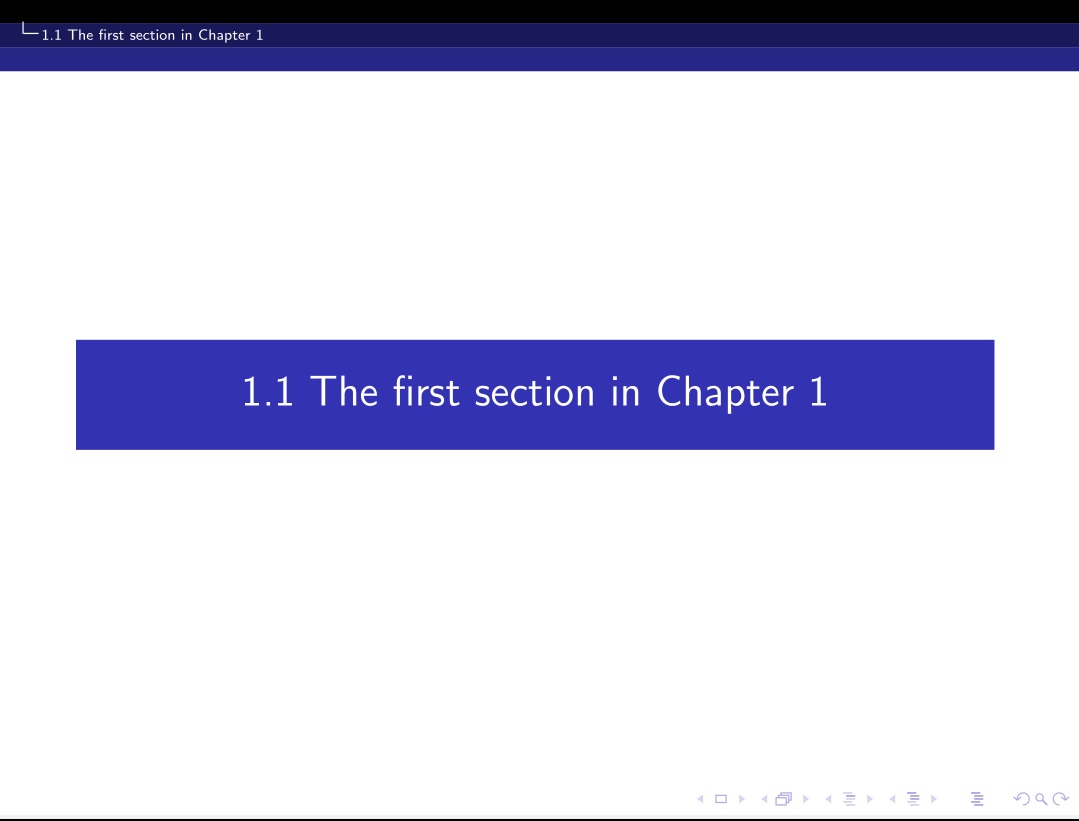
\includegraphics[width=4.26042in,height=\textheight,keepaspectratio]{images/clipboard-2994615373.jpeg}

\end{tcolorbox}

\subsection{Slide 24/25}\label{slide-2425}

\begin{figure}

\centering{


\includegraphics[width=0.7\linewidth,height=\textheight,keepaspectratio,page=24]{bean.pdf}

}

\caption{\label{fig-slide24}Slide 24}

\end{figure}%

\begin{figure}

\centering{


\includegraphics[width=0.7\linewidth,height=\textheight,keepaspectratio,page=25]{bean.pdf}

}

\caption{\label{fig-slide25}Slide 25}

\end{figure}%

\begin{tcolorbox}[enhanced jigsaw, opacitybacktitle=0.6, rightrule=.15mm, opacityback=0, breakable, titlerule=0mm, colback=white, left=2mm, leftrule=.75mm, colbacktitle=quarto-callout-tip-color!10!white, colframe=quarto-callout-tip-color-frame, toptitle=1mm, bottomtitle=1mm, coltitle=black, title=\textcolor{quarto-callout-tip-color}{\faLightbulb}\hspace{0.5em}{Tip}, bottomrule=.15mm, arc=.35mm, toprule=.15mm]

\begin{itemize}
\tightlist
\item
  Pi chart comparison may be better
\end{itemize}

\end{tcolorbox}

\subsection{Slide 29}\label{slide-29}

\begin{figure}

\centering{


\includegraphics[width=0.7\linewidth,height=\textheight,keepaspectratio,page=29]{bean.pdf}

}

\caption{\label{fig-slide29}Slide 29}

\end{figure}%

\begin{tcolorbox}[enhanced jigsaw, opacitybacktitle=0.6, rightrule=.15mm, opacityback=0, breakable, titlerule=0mm, colback=white, left=2mm, leftrule=.75mm, colbacktitle=quarto-callout-tip-color!10!white, colframe=quarto-callout-tip-color-frame, toptitle=1mm, bottomtitle=1mm, coltitle=black, title=\textcolor{quarto-callout-tip-color}{\faLightbulb}\hspace{0.5em}{Tip}, bottomrule=.15mm, arc=.35mm, toprule=.15mm]

\begin{itemize}
\item
  add chapter slide
\item
  add end slide
\end{itemize}

\end{tcolorbox}


\printbibliography



\end{document}
